\documentclass[11pt,a4paper]{article}

%\def\bibcommenthead{}%
%\usepackage[utf8]{inputenc}
\usepackage[urw-garamond]{mathdesign}
%\usepackage[T1]{fontenc}
\usepackage[tuenc]{fontspec}%
%\setmainfont{Garamond}
\usepackage{ebgaramond}
\usepackage[margin=1in]{geometry} % full-width
\usepackage{amsmath}
\usepackage{amsthm}
\usepackage{parskip}
%\usepackage{amssymb}
\usepackage{hyperref}
\hypersetup{
	unicode,
%	colorlinks,
%	breaklinks,
%	urlcolor=cyan, 
%	linkcolor=blue, 
	pdfauthor={Author One, Author Two, Author Three},
	pdftitle={A simple article template},
	pdfsubject={A simple article template},
	pdfkeywords={article, template, simple},
	pdfproducer={LaTeX},
	pdfcreator={pdflatex}
}

% Natbib
%\usepackage[sort&compress,numbers,square]{natbib}
\usepackage{natbib}
\usepackage{footnote}
\bibliographystyle{apa-good}

% Theorem, Lemma, etc
\theoremstyle{plain}
\newtheorem{theorem}{Theorem}
\newtheorem{corollary}[theorem]{Corollary}
\newtheorem{lemma}[theorem]{Lemma}
\newtheorem{claim}{Claim}[theorem]
\newtheorem{axiom}[theorem]{Axiom}
\newtheorem{conjecture}[theorem]{Conjecture}
\newtheorem{fact}[theorem]{Fact}
\newtheorem{hypothesis}[theorem]{Hypothesis}
\newtheorem{assumption}[theorem]{Assumption}
\newtheorem{proposition}[theorem]{Proposition}
\newtheorem{criterion}[theorem]{Criterion}
\theoremstyle{definition}
\newtheorem{definition}[theorem]{Definition}
\newtheorem{example}[theorem]{Example}
\newtheorem{remark}[theorem]{Remark}
\newtheorem{problem}[theorem]{Problem}
\newtheorem{principle}[theorem]{Principle}

\usepackage{graphicx, color}

%\usepackage[linesnumbered,ruled,vlined,commentsnumbered]{algorithm2e} % use algorithm2e for typesetting algorithms
\usepackage{algorithm, algpseudocode} % use algorithm and algorithmicx for typesetting algorithms
\usepackage{mathrsfs} % for \mathscr command

\usepackage{lipsum}

% Author info
\title{Testing Differences in Performance of Pricing Models}
\author{Jose Pliego San Martin}

\date{
	Department of Statistical Science, Duke University\\%
	March 2023
}

\begin{document}
\maketitle

\nocite{*}
	
\begin{abstract}
Pricing models play a very important role in the insurance industry, and companies aim to price policies correctly by predicting the costs associated to them. Gradient Boosting Machines have shown great predictive performance but, unfortunately, are often unstable. In this project, we propose repeated cross validation as a modeling pipeline that allows for a more robust estimation of model performance and adapts well to different time and computational resources. We also use a paired \textit{t-}test to assess whether differences in performance are statistically significant or not. This test is adjusted to account for the dependence present in cross validation splits.
\end{abstract}

%\tableofcontents
	
\section{Introduction}
\label{sec:intro}
Accurately pricing policies is key for insurance companies. Under-pricing policies results in losses for the company, while over-pricing policies may result in customers turning to competitors for a better quote. Gradient Boosting Machines (GBMs) have shown great predictive performance in this setting, however, they tend to be unstable. This instability mainly comes from GBMs being prone to overfitting if adequate hyperparameters are not set. However, due to the high number of hyperparameters that some of the popular implementations have, it is difficult to tune hyperparameters and prevent overfitting. Instability is an issue because it is difficult to say when one model performs better than another, and because companies are interested in keeping the policy prices relatively stable across periods to prevent client discontent and avoid regulatory issues.

Focusing on the first concern, it is important for data scientists to identify when one model is better than another. Data scientists select models based on their predictive performance. A usual modeling pipeline consists of splitting the data into three sets: a training set, a validation set, and a holdout or test set. It is common to use the training and validation sets for hyperparameter tuning and model selection, and then use the test set to get an unbiased estimate of predictive performance. However, this approach does not allow for uncertainty quantification on predictive performance.

The goal of this project is to propose repeated cross validation as a technique that allows for a more robust estimation of model performance, including some uncertainty quantification and the possibility to conduct hypothesis testing on predictive performance, while being easy to adapt to different amounts of computational and time resources. The organization is as follows. In section \ref{sec:methods} We briefly introduce gradient boosting machines, a Bayesian hyperparameter optimization library called Optuna \citep{optuna}, repeated and nested cross validation, and show the paired $t-$test proposed by \cite{ttest} to test whether differences in performance are statistically significant. In section \ref{sec:results}, we apply the methods from section \ref{sec:methods} on a public insurance dataset \citep{allstate-claims-severity}. Finally, in section \ref{sec:discussion} we mention some limitations and potential next steps for the project.

\section{Methods}
\label{sec:methods}

Boosting is a technique that combines several "weak" learners to produce a powerful classification or regression algorithm. Gradient Boosting Machines (GBMs) often use decision trees as the weak learners, similar to bagging or random forests. However, the main difference is that GBMs iteratively add decision trees to the procedure based on the performance of the previous trees. Two of the most popular libraries for GBMs are XGBoost \citep{xgboost} and LightGBM \citep{lightgbm}. They are often used as "off-the-shelf" procedures for predictive tasks with tabular data because they maintain some of the desirable properties of decision trees like ease to combine categorical and numerical predictors, being invariant to monotonic transformations of the predictor variables, and robustness to outliers while greately increasing predictive performance \citep{esl}. As mentioned in section \ref{sec:intro}, the great performance comes at a cost. Namely, GBMs are prone to overfitting without proper hyperparameter tuning. However, hyperparameter tuning is a challenging task because of the large number of tunable components (e.g., LightGBM has more than 50 tunable hyperparameters).

To aid in hyperparameter tuning, the Optuna library developed by \citet{optuna} has become increasingly popular. Optuna is a Bayesian optimization library. Without diving deep into the details, Optuna performs hyperparameter tuning by trying out configurations of the hyperparameters that yield the greatest expected decrease on the loss function. Depending on the number of hyperparameters to tune, this optimization can be very computationally expensive, but it performs a better exploration of the hyperparameter space than regular grid search since the size of the grid grows exponentially with the number of hyperparameters.

When fitting machine learning models for predictive purposes, it is of great interest for data scientists to evaluate how the models will perform in production. To get an estimation of predictive performance, a portion of the data is left out of the training procedure and only used to estimate future performance. The remaining data is usually split into a training and a validation set. A common modeling pipeline will fit and train different models on the training set, and use the validation data for model selection. However, this procedure yields a single performance observation that does not allow for uncertainty quantification around the data splitting procedure. Another disadvantage is that performance on the validation set is often used for hyperparameter tuning, which may result in the estimates being overly optimistic since information leaks during the training procedure.

A common way to get more robust estimates of performance while accounting for randomness in the data splitting procedure is cross validation (CV) \citep{esl}. $K-$fold cross validation consists of splitting the data into $k$ disjoint sets and using each of the sets as a validation set once and the other $k-1$ as a training set. In the end, this procedure yields $k$ different performance observations. The main disadvantage with cross validation is that the performance observations are not independent due to overlap in the $k$ training datasets. If we want to get many performance observations, then we need to split the data into many folds. However, splitting into many folds will results in higher variance of the performance measurements since each model is only validated in a very small portion of the data. A workaround for this issue is to perform repeated cross validation, which consists of performing $k-$fold cross validation a total of $r$ times. In the end, a total of $r \times k$ performance measurements are obtained.

When doing cross validation, we also face the issue of tuning hyperparameters on the same set in which we are measuring performance. Nested cross validation is a solution to this problem. The idea of nested cross validation is to first divide the training set using $k-$fold or $r\times k$ repeated cross validation, and within each fold, use $k-$fold cross validation again for hyperparameter tuning. This procedure, combined with the hyperparameter tuning with Optuna, can be very time and computationally expensive.

After repeated cross validation (nested or not), we can perform a paired $t-$test with the $r\times k$ performance observations of two different models. As mentioned earlier, the observations are not independent and therefore classical $t-$tests yield high type I error probabilities due to variance underestimation. The test introduced by \citet{ttest} aims to stabilize type I error probabilities by adjusting the variance estimate. The statistic used is 
\begin{equation}
\label{eq:ttest}
t = \frac{\sum_{i = 1}^r \sum_{j = 1}^k \delta_{ij}}{\sqrt{\left(\frac{1}{r\times k} + \frac{n_2}{n_1}\right)\hat{\sigma}^2}},
\end{equation}
where $r$ is the number of repeats, $k$ is the number of folds in each repeat, $n_2$ is the size of each validation set, $n_1$ is the size of the each training set, and $\delta_{ij}$ is the difference in performance between the two models fit on fold $j$ of repeat $i$. This $t-$statistic has been show through simulations to provide stable type I and type II error probabilities \citep{bouckaert}.

\section{Results}
\label{sec:results}

\begin{table}[ht]
\centering
\begin{tabular}{|c|c|c|c|}
\hline
Cross Validation & Average MAE & SD MAE & Computing Time\footnotemark{}\\
\hline
Nested Repeated CV & 1149.73 & 10.52 & 2h 35m\\
Non-nested Repeated CV & 1148.85 & 9.69 & 1h 2m\\
\hline
\end{tabular}
\caption{Comparing nested and non-nested cross validation.}
\label{tbl:cv}
\end{table}
\footnotetext{Tested using 5 cores in parallel on a 2022 MacBook Air with 8 GB RAM and M2 chip (MacOS Ventura 13.1).}

We apply the methods introduced in section \ref{sec:methods} to a Kaggle dataset \citep{allstate-claims-severity}. The data consists of 194,000 insurance claims, with 116 categorical predictors and 14 numerical predictors. The goal is to predict the severity, or the monetary costs associated with each claim. The loss function is mean absolute error (MAE) defined as $$\mathcal{L}(y, \hat{y}) = \frac{1}{n} \sum_{i=1}^n |y_i - \hat{y}_i|.$$ We use the LightGBM API and Optuna libraries in Python.

The first step is to compare the average loss estimates and standard deviation obtained with $3\times 3$ repeated cross validation, using both a non-nested and a nested approach with $3-$fold cross validation as the nested splitting method. The results are shown in table \ref{tbl:cv}. As a reference, the MAE obtained on the training data using an intercept-only model is 1969.86. We can see that the non-nested approach gives a slightly lower average MAE and standard deviation, which was expected due to the over-optimism that comes from tuning hyperparameters and evaluating on the same dataset. We can also see that the nested cross validation takes significantly more time to run. Overall, the differences observed in loss estimates make me think that the additional time required to perform nested cross validation is not really worth the extra time and computational costs.

\begin{figure}[ht]
\centering
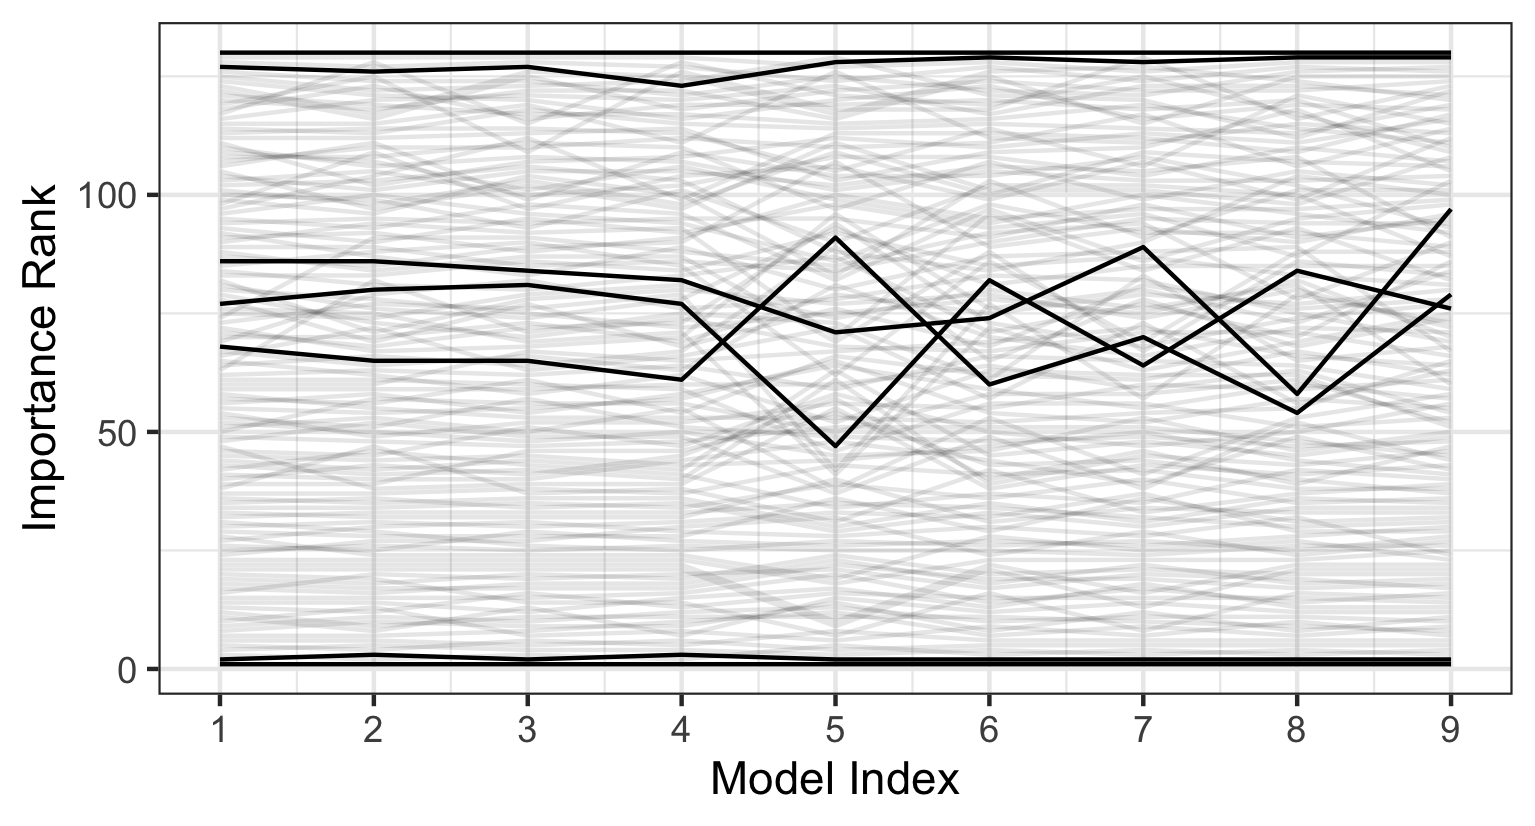
\includegraphics[width=0.7\textwidth]{importance_notitle.png}
\caption{Variable importance rankings for the nine nested cross validation models.}
\label{fig:example}
\end{figure}

Now, suppose that due to new regulations, insurance companies are not allowed to use certain client characteristics to price policies. We are interested in evaluating how the performance of our model changes when removing these predictors. We can get a sense of how performance will be affected by looking at the variable importance plots in figure \ref{fig:example}. Note that this is not a case of feature selection based on variable importance. We are assuming that regulatory authorities are forcing companies to remove some fixed subset of predictors and the variable importance plot is used solely to build intuition on how the models may be affected.

\begin{table}[ht]
\centering
\begin{tabular}{|c|c|c|c|c|}
\hline
Model & Average MAE & SD MAE\\
\hline
Full & 1146.34 & 9.46\\
Reduced & 1143.99 & 8.51\\
\hline
\end{tabular}
\caption{MAE estimates obtained with $5\times 5$ repeated cross validation.}
\label{tbl:diff}
\end{table}

If the predictors removed are not very important for the model, like the two predictors highlighted at the top of figure \ref{fig:example}, then the model may not be as hindered as if we must remove the two predictors highlighted at the bottom (the most important variables). We refit the models using $5\times 5$ repeated cross validation (non-nested) and show the results in table \ref{tbl:diff}. The reduced model actually performs better than the full model! This is a common phenomenon when using many predictors, especially when some of the predictors are high-cardinality categorical variables since their removal can serve as a form of regularization. We are then interested in testing whether the differences observed are statistically significant or if they can be attributed to the noisy procedure of splitting the data and performing hyperparameter tuning.

To test whether differences are significant, we calculate the $t-$statistic in equation \ref{eq:ttest} and compare the observed value to the 2.5 \% and 97.5 \% quantiles of a $t-$distribution with 24 degrees of freedom. Table \ref{tbl:ttest} shows the observed value for the $t-$statistic. We obtain a $p-$value greater than 0.05, meaning that there is no concrete evidence to conclude that one model is better than the other at a 5 \% level.

\begin{table}[ht]
\centering
\begin{tabular}{|c|c|c|c|c|}
\hline
Model & Average MAE & SD MAE & Average Difference & \textit{t-}statistic\\
\hline
Full & 1146.34 & 9.46 & 2.35 & 2.06\\
Reduced & 1143.99 & 8.51 & &\\
\hline
\end{tabular}
\caption{\textit{p}-value > 0.05 obtained with a $t_{r\times k-1}$ distribution.}
\label{tbl:ttest}
\end{table}

After conducting the statistical test and settling for the reduced model due it being compliant with the hypothetical new regulations and more parsimonious, we train a new model on the whole training data using the optimal hyperparameters obtained with repeated cross validation and further tuning on the test set, and use the Kaggle submission as the evaluation on a holdout set. The results are presented in table \ref{tbl:results}.

\begin{table}[ht]
\centering
\begin{tabular}{|c|c|}
\hline
Evalaution & MAE\\
\hline
Test Set & 1127.47\\
Public Kaggle & 1122.27\\
Private Kaggle & 1134.54\\
Kaggle Winner & 1109.71\\
\hline
\end{tabular}
\caption{MAE observed after further hyperparameter tuning.}
\label{tbl:results}
\end{table}

We see that the final loss estimate on the test set overestimates the public Kaggle score calculated on 30 \% of a holdout set, and underestimates the private Kaggle score calculated on the remaining 70 \%. Overall, the MAE estimates obtained using repeated cross validation are higher than the actual scores. This can be explained by the increased bias coming from training on a smaller proportion of the data during cross validation. It is important to note that the cross validation estimates were too conservative, which is usually a more desirable behavior than being too optimistic on performance estimates.

\section{Discussion}
\label{sec:discussion}

We observe that multiple performance measurements obtained with repeated cross validation can help in quantifying uncertainty and performing hypothesis tests on different models. Using the $t-$statistic proposed by \citet{ttest} we are able to account for the fact that training sets in cross validation are not independent and ususal $t-$tests yield high type I error rates.

In the example performed on a public dataset, we observe that preventing information leakage using nested cross validation does not seem to outweigh the big computational costs that come with this approach. Furthermore, we see that the loss estimates obtained with cross validation are too conservative compared to the actual performance in the holdout set. This could be attributed to the increased bias incurred when training on a small portion of the data, but it could also be explained by "easier" claims in the holdout set which the fitted model can accurately predict. This explanation is further supported by the fact that an intercept-only model results in a MAE of 1955.01 in the test set, lower than the MAE of 1969.86 using the intercept-only model in the training data.

Finally, it is important to note that repeated cross validation can be adapted to different amounts of computational resources by increasing or decreasing the number of repeats and folds. The possibility to tune hyperparameters and train models in parallel can be exploited using cross validation and hyperparameter tuning through Optuna.

For future work, it will be interesting to study how repeated cross validation can be used to study other model characteristics like variable importance for feature selection as motivated by figure \ref{fig:example}, or Shapley values for model interpretability. Another potential branch of analysis is studying how the Bayesian hyperparameter optimization scales when the number of hyperparameters increases. As mentioned in section \ref{sec:methods}, LightGBM has more than 50 tunable parameters but only six of them were tuned in this project.
	
\paragraph{Acknowledgements} This project was developed during the Summer of 2022, while the author was working as an intern Data Scientist on the Pricing Sophistication team at Liberty Mutual Insurance.

\newpage

\bibliography{portfolio}
\end{document}